\chapter*{Introduction générale}
\label{chap:intro}
\addcontentsline{toc}{chapter}{\nameref{chap:intro}}

\section{Contexte et motivations}
\label{sec:intro:contexte}
Une décision jurisprudentielle peut être définie soit comme  le résultat rendu par les juges à l'issue d'un procès, soit comme un document décrivant une affaire judiciaire. Un tel document rapporte, notamment,  les faits, les procédures judiciaires antérieures, le verdict des juges, et certaines explications associées. Dans cette thèse, nous désignons par \og décision \fg{} le document, et par  \og résultat\fg{} la conclusion, ou réponse finale des juges. Une jurisprudence\footnote{\url{http://www.toupie.org/Dictionnaire/Jurisprudence.htm}} est un ensemble de décisions rendues par les tribunaux ; elle représente la manière dont ces derniers interprètent les lois pour résoudre un problème juridique donné (type de contentieux). Les juristes doivent alors collecter ces documents, les sélectionner, et les analyser afin de mener, par exemple, des recherches empiriques en droit \citep{ancel2003expulsion, jeandidier2006pensions}. Les avocats exploitent aussi les décisions passées pour anticiper les résultats des juges. Ils peuvent ainsi mieux conseiller leurs clients sur le risque judiciaire que ces derniers encourent, et sur la stratégie à adopter pour un type de contentieux. 

Cette activité de collecte et d'analyse centrale pour de nombreux métiers du droit est aujourd'hui généralement effectuée de manière manuelle. Elles est par conséquent sujette à plusieurs difficultés notamment liées à l'accès et à l'exhaustivité des documents traités dans un contexte d'étude spécifique. Il faut ici notamment souligner que les documents sont dispersés dans les nombreux tribunaux, et que les procédures administratives ne facilitent pas toujours leur accès du fait de la nécessité de préserver la confidentialité des parties. En effet, les décisions n'étant la plupart du temps pas anonymisées, elles restent alors inaccessibles aux juristes qui en font la demande. Un certain nombre de documents sont néanmoins accessibles sur internet grâce à des sites de publication de données ouvertes gouvernementales, comme \url{http://data.gouv.fr} en France, \url{https://www.judiciary.uk} en Grande Bretagne, \url{http://www.scotusblog.com/} aux Etats-Unis, et \url{https://www.scc-csc.ca/} au Canada. Ces sites publient régulièrement des décisions récemment prononcées.  Il existe aussi des moteurs de recherche juridiques qui permettent de retrouver des décisions intéressantes. Cependant, qu'ils soient payants ( LexisNexis\footnote{\url{https://www.lexisnexis.fr/}}, Dalloz\footnote{\url{http://www.dalloz.fr}}, Lamyline\footnote{\url{http://lamyline.lamy.fr}},...) ou gratuits (CanLII\footnote{\url{https://www.canlii.org}}, Légifrance\footnote{\url{https://www.legifrance.gouv.fr}}, ...), les critères de recherche offerts par leurs moteurs de recherche d'information limitent grandement la pertinence des résultats pouvant être obtenus. En effet, il ne s'agit en général que de combinaisons de mots-clés et autres métadonnées (date, type de juridiction, ...), ou d'expressions régulières, comme l'illustre la Figure \ref{fig:intro:juriSearchForm}. Ces critères n'appréhendent pas la sémantique juridique, et ne permettent pas la plupart du temps aux juristes, sinon difficilement, la constitution d'échantillons pertinents pour leurs études. 

\begin{figure}[!htb]
	\centering
%	\begin{subfigure}[t]{0.95\textwidth}
%		\centering
%		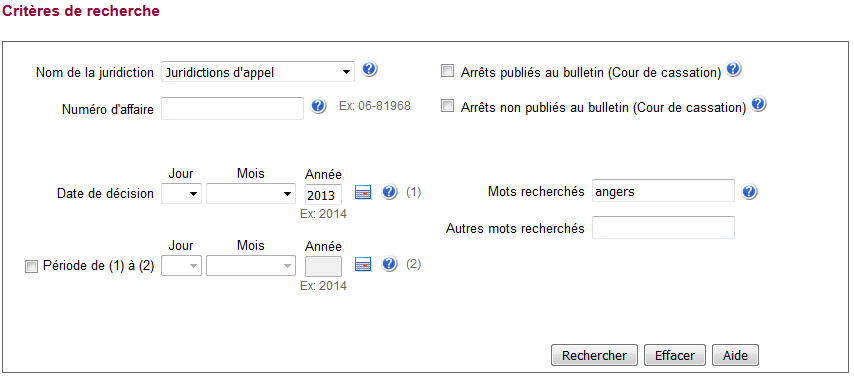
\includegraphics[width=0.9\textwidth]{legifrance.PNG}
%		\caption{Formulaire de Légifrance}
%	\end{subfigure}%

	\begin{subfigure}[t]{0.45\textwidth}
		\centering
		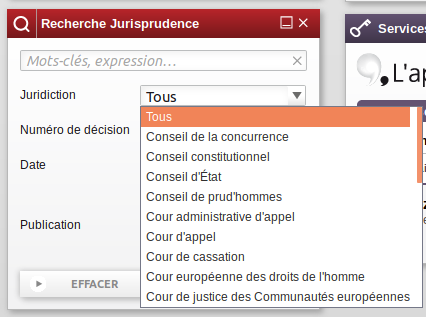
\includegraphics[scale=0.4]{dalloz.png}
		\caption{Formulaire de Dalloz}
	\end{subfigure}\hfill
	\begin{subfigure}[t]{0.55\textwidth}
		\centering
		\fbox{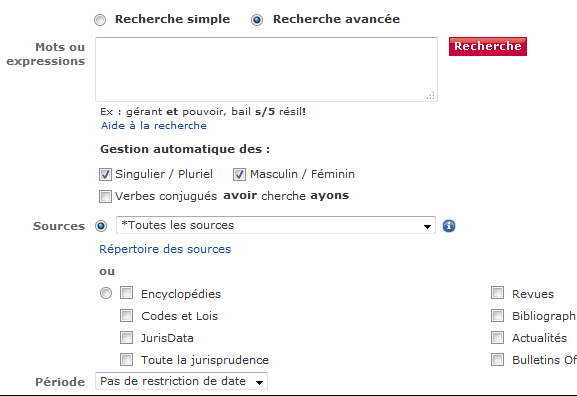
\includegraphics[scale=0.35]{lexisnexis.png}}
		\caption{Formulaire de LexisNexis}
	\end{subfigure}%
	\caption{Exemples de critères des moteurs de recherche juridique}\label{fig:intro:juriSearchForm}
\end{figure}

Plus de 4 millions de décisions sont prononcées en France par an d'après les chiffres du ministère français de la justice (Tableau \ref{tab:intro:nbdecisionstats}). Dans ce contexte, l'exhaustivité, ou tout au moins la représentativité d'une analyse menée de manière traditionnelle, manuellement, est aussi fortement limitée du fait de l'énorme volume de documents existants. 
Au regard de la croissance rapide du nombres de décisions accumulées chaque année, on imagine facilement que même une étude sur une question très précise nécessite la constitution laborieuse d'un large corpus de décisions. Par ailleurs, il peut s'avérer très pénible de lire les décisions pour en identifier les données d'intérêt. Les documents sont très souvent longs et complexes dans leur style de rédaction. Par exemple, les phrases comprennent très souvent plusieurs clauses discutant d'aspects différents. On y retrouve aussi des références à des jugements antérieurs, et des omissions.


Il est évident qu'une automatisation du traitement des corpus de décisions s'impose pour répondre aux diverses difficultés d'accès, de volumétrie, et de complexité liées à la compréhension des décisions. L'automatisation ferait gagner du temps aux juristes lors de tâches de traitement préalables à leur raisonnement d'experts, tout en leur fournissant une vue pertinente de la jurisprudence. D'autre part, \citet{cretin2014justicecomplexe} fait remarquer que la justice est complexe dans son organisation (Figure \ref{orgjusticefrance}) et son fonctionnement, et que son langage est pratiquement incompréhensible. Il est donc presque impossible pour les "profanes" d'estimer leurs droits et le risque judiciaire qu'ils encourent dans leur quotidien sans consulter un initié du droit. L'automatisation de l'analyse jurisprudentielle pourrait ainsi améliorer l'accessibilité du droit dans ce cas.  L'exigence pour le profane étant l'exacte pertinence des ressources, leur accessibilité, et l'intuitivité du processus de leur exploitation \citep{narazenko2017legalnlpintro}. Le traitement automatique de la jurisprudence constituerait alors une aide précieuse non seulement pour les professionnels du droit, mais aussi pour les particuliers et les entreprises soucieux de voir l'issue de leur affaire leur être favorable. Par exemple, en comparant le montant qu'on peut espérer d'une juridiction et le coût d'un procès, on peut plus aisément se décider entre un arrangement à l'amiable et la poursuite du litige en justice \citep{langlaischappe2009ecoresolutionlitige}. 

\begin{figure}[!htb]
	\centering 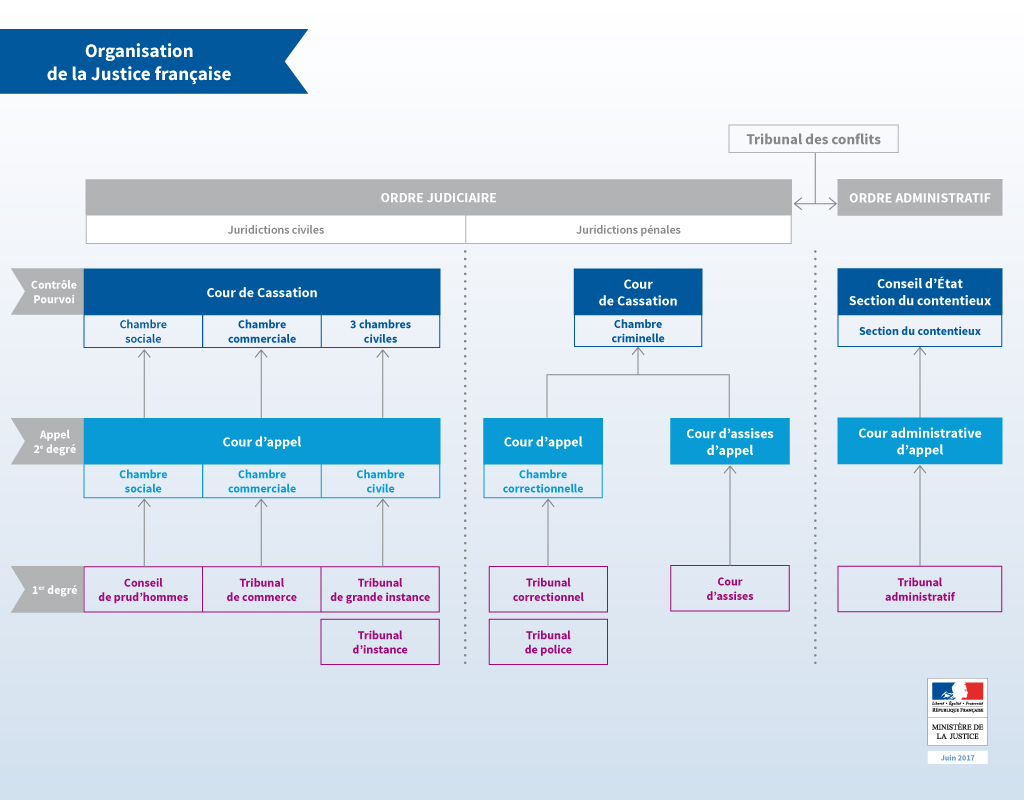
\includegraphics[width=0.9\textwidth]{organisation_justice_francaise_grand.jpg}
	
	\textit{\scriptsize{Source: \url{http://www.justice.gouv.fr/organisation-de-la-justice-10031/}}}  
	\caption{Organisation des institutions judiciaires françaises} \label{orgjusticefrance}
\end{figure}

\section{Objectifs}
%\textcolor{red}{Description d'une approche traditionnelle, exemple d'études, difficultés de ces études}
 Ce mémoire propose des stratégies et modèles visant à automatiser l'extraction d'information à partir des décisions françaises. Le but est de faciliter la constitution et l'analyse descriptive de corpus de décisions de justice. L'approche traditionnelle d'analyse d'un contentieux \citep{ancel2003expulsion} consiste à :
 \begin{enumerate}
 	\item \textbf{Choisir un échantillon représentatif}: collection des décisions suivant des contraintes définies:  période précise, couverture géographique, types d'affaires, etc.
 	\item \textbf{Sélectionner les décisions}: élimination des décisions qui ne correspondent pas au type de demande d'intérêt.
 	\item \textbf{Élaborer la grille d'analyse}: création d'un modèle de grille qui permettra d'enregistrer les informations potentiellement importantes. Chaque ligne de la grille correspond à une demande, et les colonnes font référence aux différents types d'informations qu'il est possible d'extraire sur une demande. Ces variables vont de la procédure suivie, aux solutions proposées, en passant par la nature de l'affaire. Les champs à remplir ne sont pas connus à l'avance ; ce n'est généralement qu'au cours de la lecture des décisions que l'on distingue les informations pertinentes pour l'étude.
 	\item \textbf{L'analyse des décisions et l'interprétation des informations}: saisie des décisions et calculs statistiques dans un logiciel tableur.
 \end{enumerate}
 
\citet{ancel2003expulsion} évoque principalement le problème de la différence entre l'état capté de la jurisprudence et son état présent. D'une part en effet, les longs délais de travail sont caractéristiques de ces études. Nous avons pour exemple, l'étude menée  par l'équipe de \citet{jeandidier2006pensions} pour l'analyse empirique des déterminants de la fixation de pensions alimentaires pour enfant lors de divorce. Cette analyse a duré 9 mois pour l'extraction manuelle des informations et la modélisation par régression de la relation entre les déterminants extraits et les pensions alimentaires accordées.  D'autre part, il est impossible d'observer l'évolution des pratiques judiciaires dans le temps et dans l'espace du fait de la faible taille de l'échantillon choisi. Notre principal objectif est donc de proposer des solutions pour un traitement rapide et efficace d'une grande masse de décisions. 
 
 La problématique de notre étude est de \og \textbf{capter automatiquement la sémantique d'un corpus jurisprudentiel pour comprendre la prise de décision des juges sachant que l'interprétation subjective des règles juridiques rend l'application de la loi non déterministe} \fg{}. Cette question intéresse des entreprises telles que LexisNexis, et plusieurs startups  à l'exemple de Predictice\footnote{\url{http://predictice.com}} et CASE LAW ANALYTICS\footnote{\url{http://caselawanalytics.com}}. Afin d'y répondre, nous nous intéressons aux concepts manipulés par les experts, au centre desquels nous retrouvons les demandes des parties (prétentions) qui feront l'objet d'une décision. En effet, l'analyse sémantique d'un corpus jurisprudentiel vise  la plupart du temps à identifier des connaissances sur les nombreuses demandes présentent dans les décisions. Ces demandes sont associées à plusieurs concepts importants qui enrichissent la compréhension de la décision (Figure \ref{fig:intro:demande-central}).
 \begin{figure}[!htb]
 	\centering
 	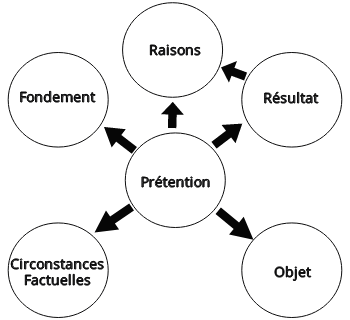
\includegraphics[scale=0.7]{demande-central.png}
 	\caption{La demande au centre de la compréhension des décisions}
 	\label{fig:intro:demande-central}
 \end{figure} 

Une demande peut ainsi être caractérisée par :
 \begin{itemize}
	\item le résultat associé qui est décrit par une polarité (\og accepte \fg{} ou \og rejette \fg{}), souvent lié à un quantum accordé, par exemple 5000 euros de dommages et intérêts ou 2 mois d'emprisonnement ;
	\item le fondement ou la norme juridique qui est la règle qui est associée et qui légitime la prétention ou le résultat ;	
	\item l'objet qui représente ce qui a été demandé (par ex. dommages et intérêts) ;
	\item les circonstances factuelles dans lesquelles sont formulées les demandes ; elles décrivent les types de faits caractérisant ainsi les types de contentieux ou d'affaires ;
	\item les divers arguments apportés par les parties (resp. les juges) pour justifier leurs requêtes (resp. leurs solutions).
 \end{itemize}

Ces concepts descriptifs d'une demande couvrent très souvent l'essentiel de l'information pertinente pour les experts. 

Les travaux de cette thèse s'inscrivent dans un projet qui vise, entre autres, à automatiser l'extraction de l'ensemble de ces informations et de les structurer afin d'enrichir une base de connaissances contenant des informations détaillées de la jurisprudence française. Une telle base permettrait notamment de mener des études sur différents critères comme la juridiction, le type de demande, ou encore les circonstances du litiges, dans différents contextes de prise de décision juridique. Elle aurait aussi tout naturellement une importance certaine pour l'étude  de la définition de modèles prédictifs variés, e.g. de l'application du droit, par exemple pour la prédiction des types de demandes à effectuer dans le cadre d'un litige. 

Le projet comprend deux phases principales : une phase d'indexation des connaissances de la masse des décisions, suivie d'une phase d'analyse prédictive. La phase d'indexation doit déjà permettre de réaliser automatiquement, de manière exhaustive, des analyses descriptives. Ces dernières consistent, par exemple, à comparer le nombre d'acceptations à la fréquence des rejets. Par conséquent, le système doit apprendre à reconnaître dans les décisions, les informations pertinentes sur les prétention et résultats associés. La phase d'analyse consiste à regrouper des paquets de décisions similaires (même résultat sur la même prétention dans les circonstances similaires), pour découvrir les facteurs influençant le sens du résultat (par ex. le fait que \og le revenu de l'époux soit le plus élevé du foyer\fg{} encourage les juges à accorder la pension alimentaire à l'épouse). En effet, c'est la connaissance de ces factuels circonstanciels démunis de toute teneur juridique qui permet à l'expert de pouvoir anticiper les décisions judiciaires.

 La chaîne de traitement à mettre en \oe uvre se compose de quatre étapes principales qui s'enchaînent comme le présente la figure \ref{fig:intro:pipeline-globale}. Notre étude s'intéresse donc aux problématiques liées la constitution de la base de connaissance et à son exploitation dans un contexte d'analyses descriptives. Celles-ci sont décrites dans la suite.
\begin{figure}
	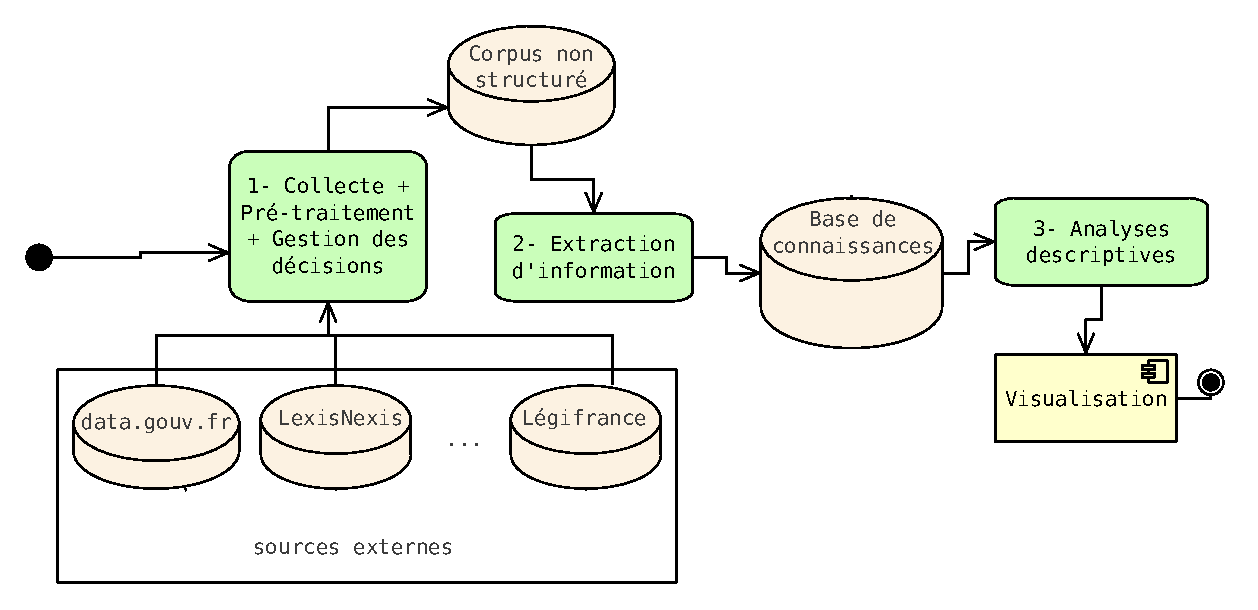
\includegraphics[width=\textwidth]{pipeline-cassandra.pdf}
	\caption{Chaîne d'analyse du corpus jurisprudentiel à mettre en \oe uvre} \label{fig:intro:pipeline-globale}
\end{figure} 


\subsection{Collecte, gestion et pré-traitement des documents}

 Le volume de décisions prononcées croît très rapidement (Tableau \ref{tab:intro:nbdecisionstats}). 
 
 \begin{table}[!htb]
 	\small
 	\begin{center}
 		\begin{tabular}{|l|l|l|l|l|l|}
 			\hline
 			\textbf{Justice}	& \textbf{2013}      & \textbf{2014}      & \textbf{2015}      & \textbf{2016}      & \textbf{2017}      \\ \hline
 			civile         & 2 761 554 & 2 618 374 & 2 674 878 & 2 630 085 & 2 609 394 \\ \hline
 			pénale         & 1 303 469 & 1 203 339 & 1 206 477 & 1 200 575 & 1 180 949 \\ \hline
 			administrative & 221 882   & 230 477   & 228 876   & 231 909   & 242 882   \\ \hline
 		\end{tabular}
 		
 		\textit{\scriptsize{Source: \url{http://www.justice.gouv.fr/statistiques-10054/chiffres-cles-de-la-justice-10303/}}}  
 	\end{center}
 	\caption{Nombre de décisions prononcées en France par an de 2013 à 2017}\label{tab:intro:nbdecisionstats}
 \end{table}
 
 Il est donc nécessaire de trouver des moyens pour collecter le maximum de documents bruts non-structurés, les pré-traiter, et organiser leur gestion afin de les indexer en local pour faciliter leur traitement. Les décisions de cours d'appel de justice civile sont les plus accessibles à partir des moteurs de recherche juridique (LexisNexis, Dalloz, LamyLine, Legifrance, etc.) et de la grande base de données JuriCa de la Cour de cassation. Cependant, l'accès à ces décisions est généralement payant et le nombre de documents simultanément téléchargeables est très faible sur les sites payants (généralement 10 à 20 décisions au maximum à la fois). De plus, le nombre de téléchargements par jour est limité. La base JuriCa est la plus grosse base de décisions de cours d'appel en France. Elle est gérée par la Cour de cassation. L'accès à cette base est offert par le Service de Documentation, des Etudes et du Rapport\footnote{\url{https://www.courdecassation.fr/institution_1/composition_56/etudes_rapport_28.html}} (SDER). L'accès est payant pour les professionnels et gratuit pour les universités et centres de recherche en partenariat avec le SDER. Légifrance, le moteur de recherche du ministère de la justice, fournit quant à lui un accès public et gratuit à un nombre considérable de documents. Les décisions y sont identifiées à l'aide de numéros consécutifs et accessibles à partir d'un service web. Ce dernier a l'avantage de proposer des décisions de tous les ordres et de tous les degrés. Cependant, les décisions des juridictions du premier degré (appelées jugements) restent plus rares sur internet et principalement disponibles auprès des tribunaux.  La disponibilité des décisions du second degré ou d'appel (appelées arrêts) en justice civile est l'une des raisons pour lesquelles notre étude s'est portée sur celles-ci.

Les décisions existent sous divers formats PDF, DOC, DOCX, RTF, TXT, XML, etc. Il arrive parfois qu'un fichier téléchargé comprenne plusieurs décisions (sur LexisNexis par exemple). Nous avons par conséquent préféré convertir tous les documents au format plein texte pour homogénéiser les traitements. Par ailleurs, les décisions sont collectées à partir de diverses sources pouvant contenir des documents identiques. Il se pose donc un problème d'identification unique des décisions pour éviter des redondances. Pour cela, nous avons défini une convention de nommage des fichiers. Ce dernier repose sur 3 informations: le type de juridiction (tribunal, cour d'appel, ...), la ville, et le numéro R.G. (registre général) qui est l'identifiant unique de la décision au sein de la juridiction. Par exemple, le numéro \og CAREN1606137 \fg{} identifie la décision de numéro R.G. \og 16/06137 \fg{} de la cour d'appel (\og CA \fg{}) de la ville de Rennes (\og REN \fg{}). Ces 3 informations sont présentes dans les premières lignes de la décision, et sont facilement identifiables à l'aide d'une routine à base de règles simples. D'autre part, certains moteurs de recherche ne fournissent souvent qu'un résumé au lieu du contenu original des décisions. Il est important de supprimer ces fichiers du corpus.

\subsection{Extraction de connaissances}
\label{subsec:intro:ie}
Les problématiques d'extraction de connaissances constitue la pierre angulaire de cette thèse car les informations sur les demandes, les parties, les juges, les juridictions et les faits conditionnent la qualité des prévisions du sens du résultat pour un type de demande considéré.  La difficulté découle de l'état non-structuré des documents, et de la complexité et la spécificité du langage employé. L'extraction des connaissances nécessite de mettre en \oe uvre des techniques de fouille de textes adaptées à la nature des éléments à identifier. Nous avons ainsi abordé l'annotation des références de l'affaire (juridiction, ville, participants, juges, date, numéro R.G., normes citées, ...), l'extraction des demandes et résultats correspondants, et l'identification des circonstances factuelles.

Les métadonnées de référence sont des segments de texte qu'on peut directement localiser dans le document. Leur reconnaissance est donc semblable à celle des entités nommées. C'est une problématique intensivement étudiée en traitement automatique du langage naturel \citep{yadav2018surveyNeuralNER} dans plusieurs travaux et compétitions, aussi bien pour des entités communes \citep{tjong2003introCoNLL,grishman1996muc6}, que pour des entités spécifiques à un domaine \citep{kim2004bioNer, persson2012nbbioner,hanisch2005prominer}, et dans diverses langues \citep{li2018wcpbioner,alfred2014malayner,amarappa2015kannada}. 

Le problème d'extraction des demandes et de la réponse correspondante des juges consiste à reconnaître pour chaque prétention : son objet, son fondement, le quantum demandé, le sens du résultat, et le quantum accordé. La paire demande-résultat s'apparente donc à des entités structurées comme les évènements \cite{ace2005event} qui sont décrits par un type, un terme-clé, des participants, un temps, une polarité.

Le problème d'identification des circonstances factuelles consiste à constituer des regroupements de décisions mentionnant une certaine catégorie de demande (objet+fondement). Le but est, comme indiqué précédemment, de repérer les différentes situations dans lesquelles cette catégorie de demande est formulée. Chacun des groupes représente donc une situation particulière partagée par les membres du groupe mais bien distinctes de celles reflétées par les autres groupes. Ce problème évoque des problématiques de similarité entre texte, de regroupement non supervisé (\textit{clustering}), et de \og modélisation thématique \fg{} (\textit{topic modeling}).  La similarité pourra faire l'objet, dans un travail futur, d'identification des raisons

A l'issue du processus d'extraction, les données extraites sont destinées à enrichir progressivement une base de connaissances. La structuration des données au sein d'une base facilite les diverses analyses automatiques applicables aux décisions et demandes judiciaires. 

\subsection{Analyse descriptive}
L'analyse descriptive exploite l'ensemble des connaissances extraites et organisées pour répondre aux diverses questions que l'on pourrait se poser sur l'application de la loi. Il est intéressant par exemple de comparer les fréquences de résultats positifs et négatifs pour une catégorie de prétention donnée dans une situation précise. Les quanta extraits servent à visualiser les différences entre les montants accordés et réclamés. D'autres analyses plus complexes permettraient d'étudier l'évolution dans le temps et les différences dans l'espace de l'opinion des juges.


\section{Méthodologie}
\label{sec:intro:methodologie}

Comme illustrées précédemment (\ref{subsec:intro:ie}), les problématiques propres aux textes juridiques trouvent généralement des analogies avec les problèmes d'analyse de données textuelles. Ainsi, les méthodes issues de l'énorme progrès réalisé dans ce domaine sont applicables aux textes juridiques. Cependant, quelques adaptations sont généralement nécessaires pour obtenir des résultats de bonne qualité hors des domaines pour lesquels ces approches ont été développées \citep{Waltl2016lexia}. De plus, la recherche en fouille de textes est souvent réalisée sur des échantillons qui ne reflètent pas toujours la complexité des données réelles. Effectuant l'une des premières études d'analyse sémantique des décisions françaises, nous avons axé notre travail sur le rapprochement des problèmes liés à l'analyse des décisions jurisprudentielles à ceux généralement traités en analyse de textes. Il s'agit ensuite d'établir des protocoles d'évaluation et d'annotation manuelle de données. Selon les problématiques identifiées et les protocoles d'évaluations définis, des méthodes adaptées ont été proposées et expérimentées sur les données réelles annotées par des experts.

\section{Résultats}
\label{sec:intro:résultats}
Une chaîne de traitement pour le sectionnement et l'annotation des métadonnées est proposée. L'applicabilité de deux modèles probabilistes, les champs aléatoires conditionnels ou CRF (\textit{conditional random fields}) et les modèles cachés de Markov ou HMM (\textit{hidden Markov Model}), est étudiée en considérant plusieurs aspects de la conception des systèmes d'extraction d'entités nommées. Le sectionnement a pour but d'organiser l'extraction des informations qui sont réparties dans des sections selon leur nature. 

Par la suite, nous proposons une méthode d'extraction des demandes et résultats en fonction des catégories présentes dans la décision. L'approche consiste en effet à identifier dans un premier temps les catégories présentes (objet+fondement) par classification supervisée. Un vocabulaire d'expression des demandes et résultats est exploité pour identifier les passages. Puis à l'aide de termes propres à chacune des catégories identifiées, les trois attributs (quantum demandé, sens du résultat, quantum accordé) des paires demande-résultat sont reconnus. 

Par ailleurs, nous analysons l'extraction particulière du sens du résultat par classification binaire des documents. L'objectif est de s'affranchir de l'identification préalable de l'expression des demandes et résultats. En effet, les décisions comprenant des demandes d'une catégorie donnée semblent ne contenir, dans une forte proportion, qu'une seule demande. Nous pensons qu'il n'est par conséquent pas nécessaire d'identifier l'expression de cette dernière pour en déterminer le sens. A partir d'une représentation adéquate du contenu de la décision, il est possible de classer cette dernière à l'aide d'un modèle de classification supervisée de documents.

L'identification des circonstances factuelles, quant à elle, est modélisée comme une tâche de regroupement non supervisée des décisions. Nous proposons dans ce cas une méthode d'apprentissage d'une métrique de dissimilarité sémantique entre textes, à l'aide d'un modèle adéquat de régression. Nous analysons différents modèles de régression. La métrique apprise a été comparée à d'autres distances établies en recherche d'information.

\section{Structure de la thèse}
\label{sec:intro:organisation}

La thèse est organisée en 6 chapitres. Le chapitre \ref{chap:literature} positionne nos travaux par rapport à ceux qui ont été réalisés précédemment sur des problématiques proches. Le chapitre \ref{chap:structuration} présente les architectures et modèles proposés pour la structuration des décisions et la reconnaissance des entités juridiques ; il discute notamment des différents résultats empiriques obtenus par application des modèles CRF et HMM. Ensuite, le chapitre \ref{chap:quanta} détaille le problème  d'extraction des paires demande-résultat, puis présente notre méthode et les résultats obtenus sue cette tâche. Le chapitre \ref{chap:sensresultat} traite de l'extraction du sens du résultat par classification directe des décisions, cela en comparant différents algorithmes et méthodes de représentation des textes. Le chapitre \ref{chap:similarite} présente notre approche d'apprentissage de la métrique de similarité textuelle, et la compare à des métriques établies en recherche d'information sur le problème d'identification des circonstances factuelles. Enfin, le chapitre \ref{chap:demo} présente les résultats de scénarios d'analyses descriptives pour illustrer l'exploitation potentielle de nos propositions sur des corpus de décisions de grande taille. 
